\documentclass{article}
\usepackage[utf8]{inputenc}
\usepackage{geometry}
\geometry{a4paper, top=15mm, bottom=20mm, left=20mm, right=20mm}
\usepackage{tzplot}
\usepackage{amsmath}
\usepackage[utopia]{mathdesign}
\usepackage{kinematikz}
\usepackage{tasks}
\newcommand{\ans}{\textcolor{red!95}{\textit{\quad}}}
%\newcommand{\ans}{\textcolor{red!95}{\textit{\quad Ans.}}}

\title{Module-Test-9\\(Physics-NEET)}

%\usepackage[italicdiff]{physics}
\usepackage{physunits}
\usepackage{multicol}
\tikzstyle test-paper=[>=latex, thick]
\tikzset{
>=latex
}
\tikzstyle{block}=[rectangle,draw, thick, minimum size=8mm, node distance=1.8cm]
\tikzstyle{pulley}=[circle,draw, thick, minimum size=10mm, node distance=1.8cm]

\tikzstyle{sblock}=[rectangle,draw, thick, minimum size=8mm, node distance=1.8cm]
\tikzstyle{spulley}=[circle,draw, thick, minimum size=8mm, node distance=1.8cm]

\tikzstyle{lblock}=[rectangle,draw, thick, minimum size=12mm, node distance=1.8cm]
\tikzstyle{lpulley}=[circle,draw, thick, minimum size=12mm, node distance=2cm]

\tikzstyle{hblock}=[rectangle,draw, thick, minimum height=12mm, minimum width=20mm, node distance=1.8cm]
\tikzstyle{Hblock}=[rectangle,draw, thick, minimum height=12mm, minimum width=24mm, node distance=1.8cm]
\tikzstyle{lift}=[rectangle,draw, thick, minimum height=60mm, minimum width=50mm, node distance=1.8cm]

\tikzstyle{Bpulley}=[circle,draw, thick, minimum size=20mm, node distance=1.8cm]

\tikzstyle{plank}=[rectangle,draw, thick, minimum height=8mm, minimum width=50mm, node distance=1.8cm]



\begin{document}
\maketitle
\noindent

\begin{center}
\textbf{Section-A}\\[4 mm]
There are 35 questions in this section. All are compulsory to do.\\[4 mm]
\end{center}

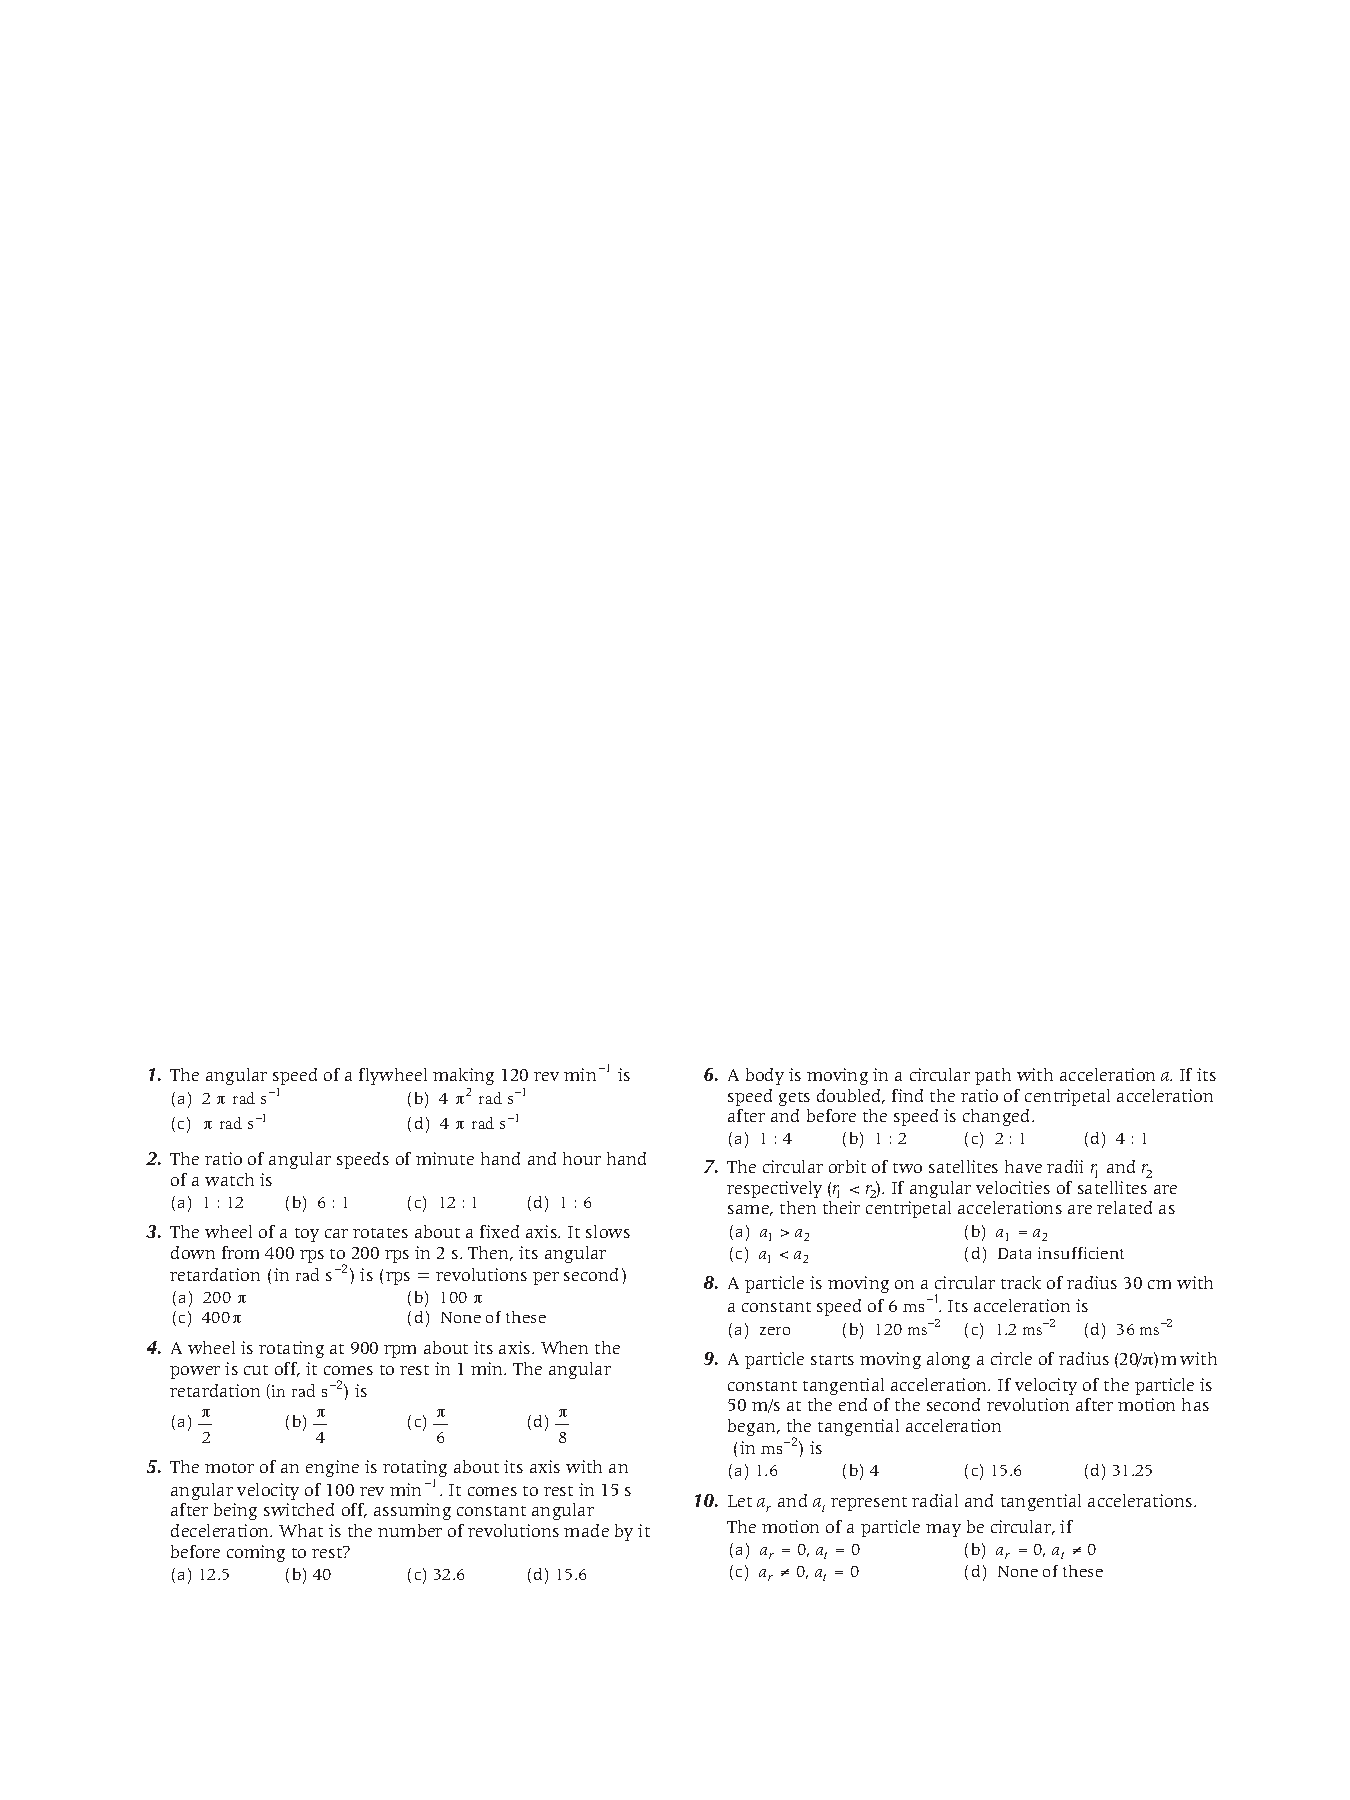
\includegraphics[trim={0.25cm 0 0 0},clip, width=170 mm]{1-10}
\linebreak
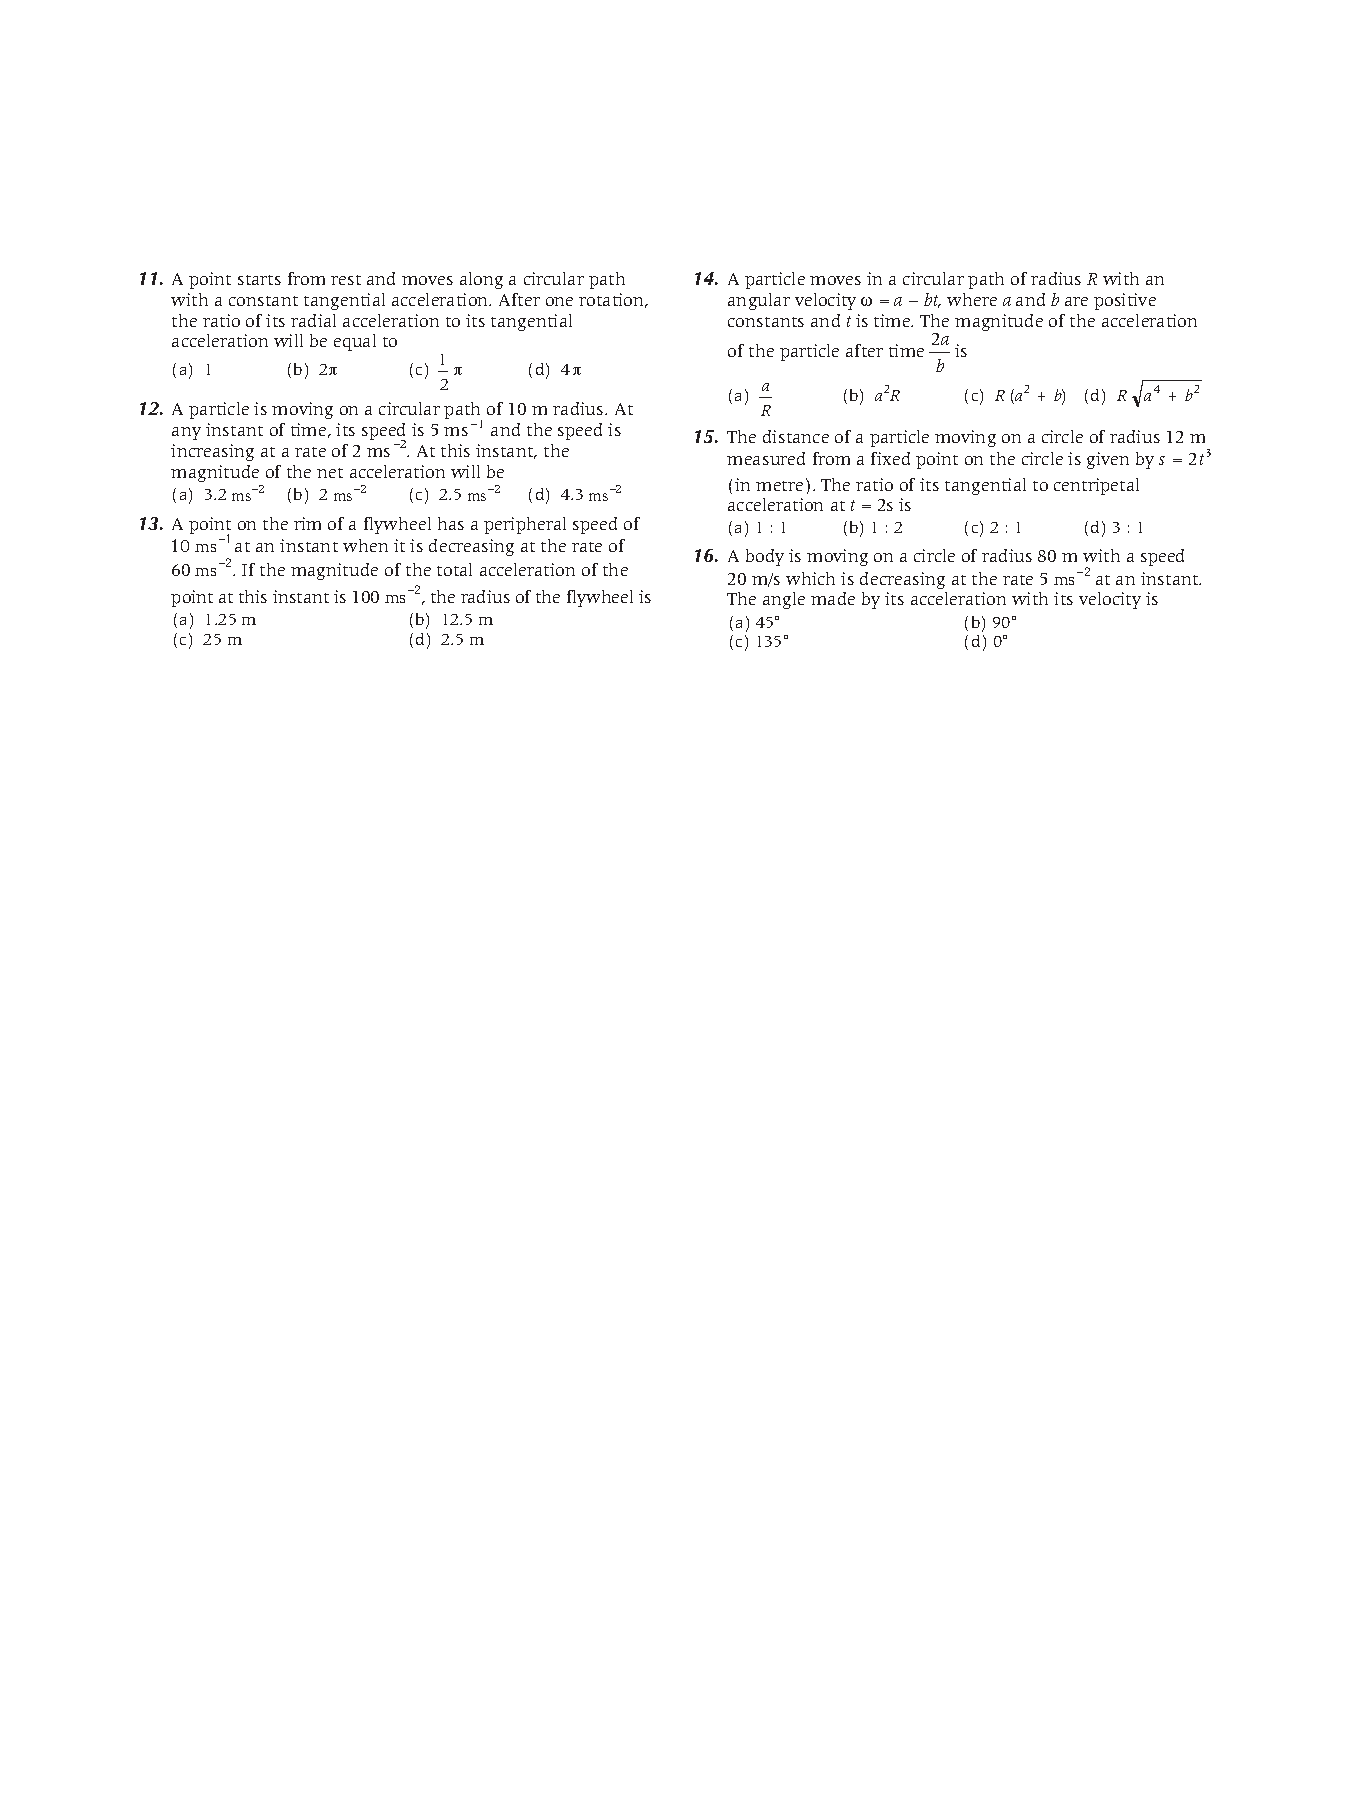
\includegraphics[trim={0 0 0 0},clip, width=170 mm]{11-16}
\linebreak
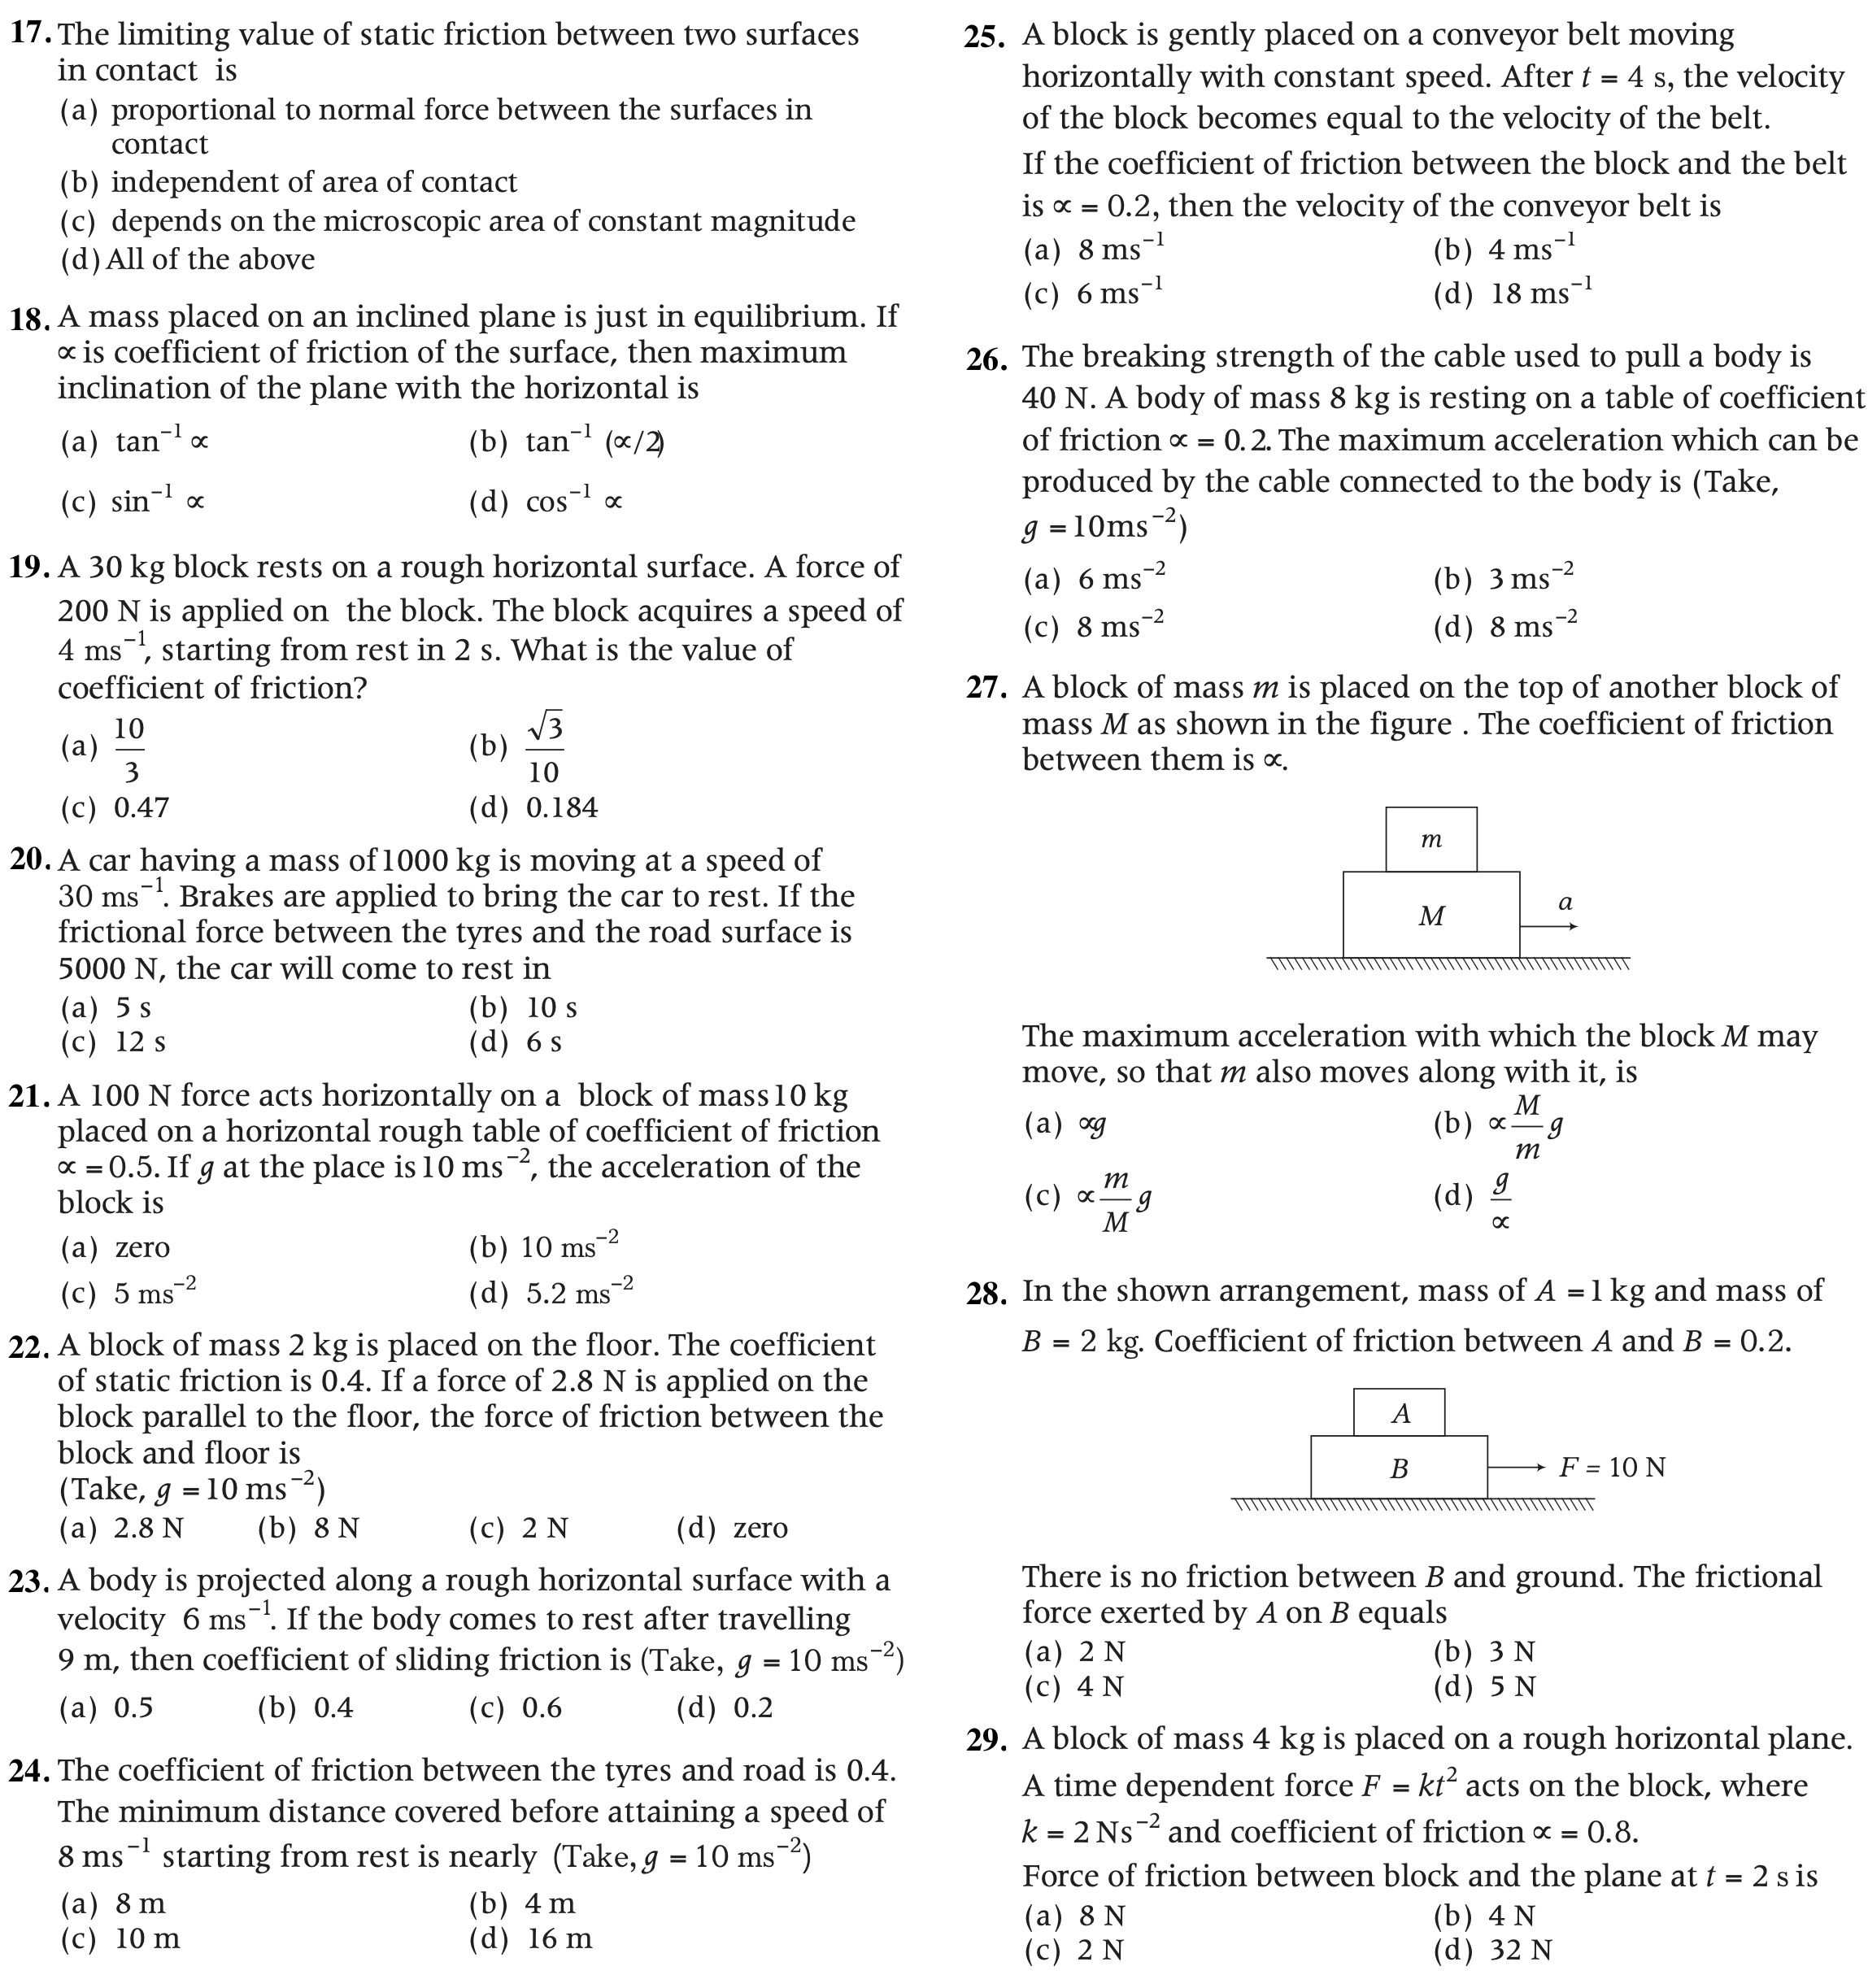
\includegraphics[trim={0 0 0 0},clip, width=170 mm]{17-29.png}
\linebreak
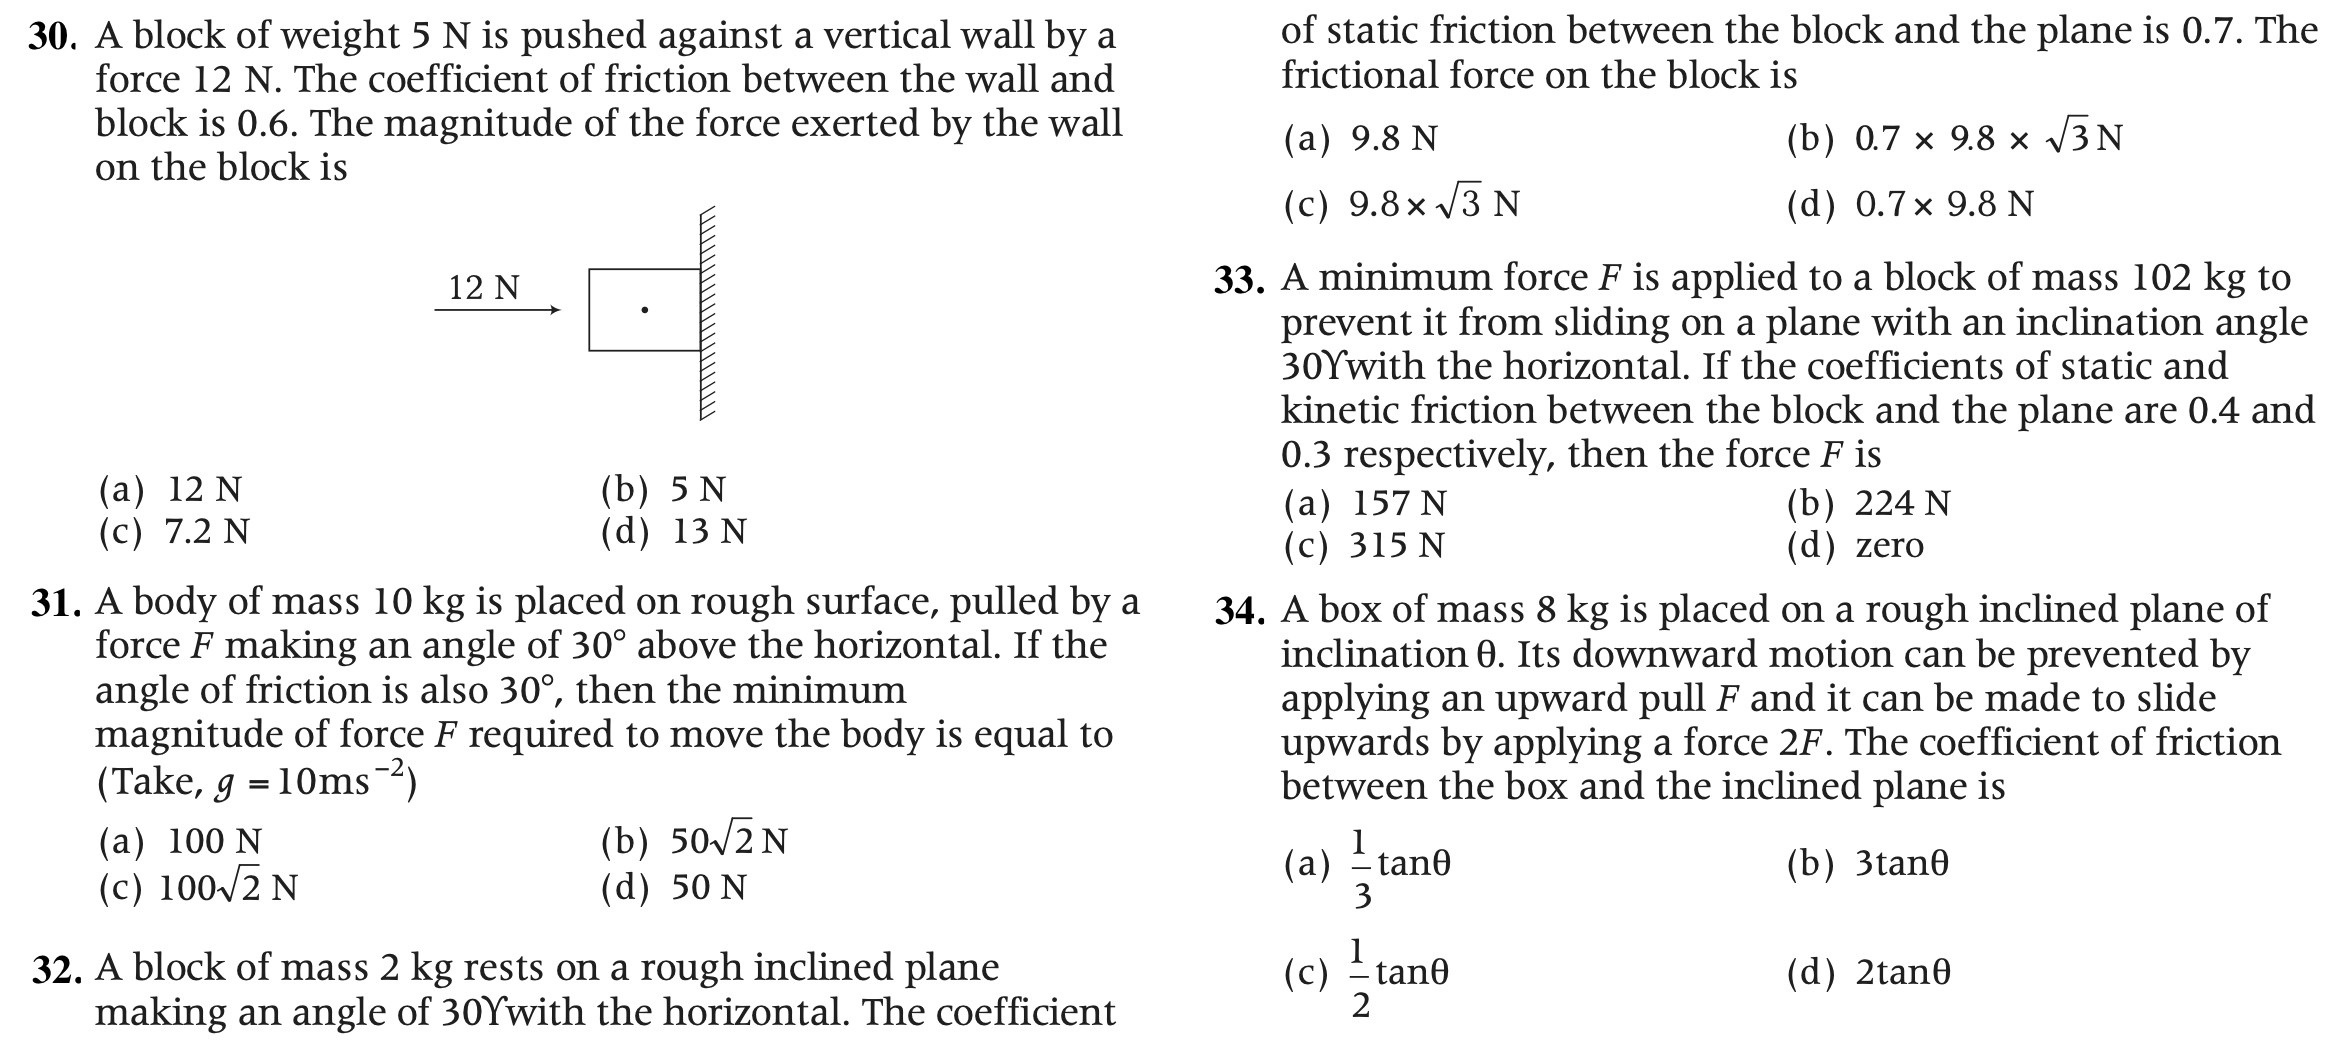
\includegraphics[trim={0 0 0 0},clip, width=170 mm]{30-34.png}
\linebreak
\begin{enumerate}



\item[35.] Which of the following statement(s) is/are true for a particle moving in a circle with a constant angular acceleration ?
\begin{enumerate}
\item The magnitude of acceleration is constant
\item The acceleration vector is along the tangent to the circle
\item The velocity vectors points along tangent to the circle
\item The velocity and acceleration vectors are always perpendicular to each other.
\end{enumerate}

\end{enumerate}

\vspace*{5mm}

\begin{center}
\textbf{Section-B}\\
There are 15 questions in this section. Only 10 questions are required to do.\\
\end{center}

\begin{enumerate}

\item A cyclist moves uniformly on a horizontal circular track of radius $100m$. If the coefficient of friction is $0.1$. At which of the following speed(s) can he travel without slipping:
\begin{tasks}(2)
\task $5 m/s$
\task $9 m/s$
\task $14 m/s$
\task None of these
\end{tasks}


\item What is the average angular speed of the second hand on a clock (in rad/s) ?
\begin{tasks}(2)
\task $6.28$
\task $0.105$
\task $0.0167$
\task $1.745 \times 10^{-3}$
\end{tasks}



\item A bicycle wheel starts at rest and has a constant angular acceleration $\alpha$. At time $t$, it has rotated through an angle $\theta$ and has an angular velocity $\omega$. What are $\omega$ and $\alpha$ in terms of $\theta$ and $t$ :
\begin{tasks}(2)
\task $\omega = \dfrac{\theta}{t}$, $\alpha=\dfrac{\theta}{t^2}$
\task $\omega = \dfrac{2\theta}{t}$, $\alpha=\dfrac{2\theta}{t}$
\task $\omega = \dfrac{2\theta}{t}$, $\alpha=\dfrac{2\theta}{t^2}$
\task None of these
\end{tasks}

\item In figure particle is shown travelling counter-clockwise in circle of radius $10 m$. The acceleration vector is indicated at a specific time. Find the value of $`v$' at this time.
\begin{multicols}{2}
\begin{enumerate}
\item $10m/s$
\item $15 m/s$
\item $20 m/s$
\item $7 m/s$
\end{enumerate}
\end{multicols}

\item A car travels at a constant speed around a circular track whose radius is $3.6 km$. The car goes once around the track in $60s$. What is the approximate magnitude of the acceleration of the car towards the centre of the track at any instant ?
\begin{multicols}{2}
\begin{enumerate}
\item zero
\item $40m/s^2$
\item $20 m/s^2$
\item $10 m/s^2$
\end{enumerate}
\end{multicols}

\item A particle is moving on a circle of radius $1 m$ and its speed is changing as $v=2t$. The magnitude of the acceleration of particle at $t=1 s$, is :
\begin{multicols}{2}
\begin{enumerate}
\item $4 m/s^2$
\item $2 m/s^2$
\item $2\sqrt{3}m/s^2$
\item $2\sqrt{5}m/s^2$
\end{enumerate}
\end{multicols}

\item A jet of water hits a flat stationary plate perpendicular to its motion. The jet ejects $500\gm$ of water per second with a speed of $1 \mps$. Assuming that after striking, the water flows parallel to the plate, then the force exerted on the plate is
\begin{tasks}(2)
	\task $5\N$
	\task $1\N$
	\task $0.5\N$\ans
	\task $10\N$
\end{tasks}

\item A force $F_1$ accelerates a particle from rest to a velocity $v$. Another force $F_2$ decelerates the same particle from $v$ to rest, then
\begin{tasks}(1)
	\task $F_1$ is always equal to $F_2$\ans
	\task $F_2$ is greater than $F_1$
	\task $F_2$ may be smaller than, greater than or equal to $F_1$
	\task $F_2$ cannot be equal to $F_1$
\end{tasks}

\item A block of mass $4 \kg$ is placed on a rough horizontal plane. A time dependent horizontal force $F = kt$ acts on the block. Here $k = 2 \N/\s$. The frictional force between the block and plane at
time $t = 2\s$ is ($\mu = 0.2$)
\begin{tasks}(2)
	\task $4\N$
	\task $8\N$\ans
	\task $12\N$
	\task $10\N$
\end{tasks}


\item Convert $60 \rpm$ into $\text{rad}/\s$ .
\begin{tasks}(2)
	\task $2\pi$\ans
	\task $4\pi$
	\task $60\pi$
	\task $120\pi$
\end{tasks}

\item Tangential acceleration is caused by 
\begin{tasks}(2)
	\task increasing radial acceleration
	\task increasing tangential speed\ans
	\task increasing angular displacement
	\task None of these
\end{tasks}

\item A particle is performing a circular motion and its angular displacement is changing as $\theta=t^2-2t$, then its angular velocity at $t=1\s$ is
\begin{tasks}(2)
	\task zero\ans
	\task Non-zero
	\task couldn't be found
	\task None of these
\end{tasks} 

\item A particle is moving on a circular track with constant speed then, which of the following statement is true?
\begin{tasks}(2)
	\task $a_t = 0$\ans
	\task $a_r = 0$
	\task $v_t = 0$
	\task None of these
\end{tasks}

\item What is the linear velocity, if angular velocity vector $\vec{\omega}=3\hat{i}-4\hat{j}+k$ and position vector $\vec{r}=5\hat{i} -6\hat{j} +6\hat{k}$ ?
\begin{tasks}(2)
	\task $6\hat{i} + 2\hat{j} -3\hat{k}$
	\task $-18\hat{i}-13\hat{j}+2\hat{k}$\ans
	\task $18\hat{i}+13\hat{j}-2\hat{k}$
	\task $6\hat{i}-2\hat{j}+8\hat{k}$
\end{tasks}

\item A ball of mass $m$ moving with velocity $v_0$ collides a wall as shown in figure. After impact it rebounds with a velocity $\dfrac{3}{4}v_0$. The impulse acting on ball during impact is
\begin{center}
\begin{tikzpicture}
\tzline+[->](1, 0)(1, 0){$x$}[r]
\tzline+[->](1, 0)(0, -1){$y$}[b]
\pic[rotate=90] {frame=4cm};
\tzline+[dashed](0, 0)(-2, 0)
\coordinate  (a) at (-2, 1.5);
\coordinate  (b) at (-2, -2.6);
\tzdot*(a)(10pt)
\tzdot*(b)(10pt)
\tzline[-->--](a)(0, 0)
\tzline[-->--](0, 0)(b)
\tzanglemark(a)(0, 0)(-2, 0){$37^\circ$}(15pt)
\tzanglemark(-2, 0)(0, 0)(b){$53^\circ$}(18pt)
\end{tikzpicture}
\end{center}
\begin{tasks}(2)
	\task $-\dfrac{1}{2}mv_0\hat{j}$
	\task $-\dfrac{3}{4}mv_0\hat{i}$
	\task $-\dfrac{5}{4}mv_0\hat{i}$\ans
	\task None of these
\end{tasks}



\begin{center}
\begin{tikzpicture}
\tzline(0, 0)(8, 0)
\tzline<0, -0.05>(0, 0)(8, 0)
\end{tikzpicture}
\end{center}

            
	
\end{enumerate}


\pagebreak

\begin{center}
\texttt{ANSWER}
\end{center}

\begin{center}
\textbf{Section-A}
\end{center}
\begin{tasks}[label=\arabic*.](2)
\task (d)
\task (c)
\task (a)
\task (a)
\task (a)
\task (d)
\task (c)
\task (b)
\task (d)
\task (c)
\task (d)
\task (a)
\task (a)
\task (d)
\task (b)
\task (c)
\task (d)
\task (a)
\task (c)
\task (d)
\task (c)
\task (a)
\task (d)
\task (a)
\task (a)
\task (b)
\task (a)
\task (a)
\task (a)
\task (d)
\task (d)
\task (a)
\task (a)
\task (a)
\task (c)
\end{tasks}

\begin{center}
\textbf{Section-B}
\end{center}
\begin{tasks}[label=\arabic*.](2)
\task (d)
\task (b)
\task (c)
\task (c)
\task (b)
\task (d)
\task (c)
\task (a)
\task (b)
\task (a)
\task (b)
\task (a)
\task (a)
\task (b)
\task (c)
\end{tasks}




\end{document}
